\documentclass[12pt,pdf,hyperref={unicode}]{beamer}
%\usetheme{boxes}
\beamertemplatenavigationsymbolsempty
\setbeamertemplate{footline}[page number]
% Set it for the internal PhD thesis defence to reduce number of slides
%\setbeamersize{text margin left=0.5em, text margin right=0.5em}

\usepackage[utf8]{inputenc}
%\usepackage[english, russian]{babel}
\usepackage{bm}
\usepackage{multirow}
\usepackage{ragged2e}
\usepackage{indentfirst}
\usepackage{multicol}
\usepackage{subfig}
\usepackage{amsmath,amssymb}
\usepackage{enumerate}
\usepackage{mathtools}
\usepackage{comment}
\usepackage[all]{xy}
\usepackage{tikz}
\usetikzlibrary{positioning,arrows}
\tikzstyle{name} = [parameters]
\definecolor{name}{rgb}{0.5,0.5,0.5}

%\usepackage{caption}
%\captionsetup{skip=0pt,belowskip=0pt}

%\newtheorem{theorem}{Theorem}
%\newtheorem{statement}{Statement}
%\newtheorem{definition}{Definition}

% colors
\definecolor{darkgreen}{rgb}{0.0, 0.2, 0.13}
\definecolor{darkcyan}{rgb}{0.0, 0.55, 0.55}
%\AtBeginEnvironment{figure}{\setcounter{subfigure}{0}}
%\captionsetup[subfloat]{labelformat=empty}

%----------------------------------------------------------------------------------------------------------

\title{ Put the title of your thesis \\ here}
%\author{Name Surname}
%\institute[]{}
%\date{2024}

%---------------------------------------------------------------------------------------------------------
\begin{document}
%\begin{frame}
%\titlepage
%\end{frame}
\setcounter{page}{1}%remove here for the title
%----------------------------------------------------------------------------------------------------------
%\section{Please do not use sectioning in the presentations}
\begin{frame}{Perplexity experiment}
 Explore the distribution of the perplexity and mean token enthropy of the Llama-3.1-8B-Instruct logits depending on the model of the generated texts.
\begin{block}{The problem}
to investigate the distribution of metrics. $PPL  = \exp\left(-\frac{1}{N} \sum_{i=1}^{N} \log P(w_i | w_{<i})\right)$, $H = -\frac{1}{N} \sum_{i=1}^{N} \sum_{j} P(w_j | w_{<i}) \log P(w_j | w_{<i})$
\end{block}
\begin{block}{The solution}
\begin{enumerate}[1)]
\item Prepare the Llama-3.1-8B-Instruct, take a part of the M4GT dataset, select the text domain,
\item Calculate perplexity and MTE metrics for model context logs on prepared texts,
\item Plot the distribution of texts by metrics on a graph, look at the average values of metrics for different models.
\end{enumerate}
\end{block}
\end{frame}
%----------------------------------------------------------------------------------------------------------
\begin{frame}{Distribution for reddit data}
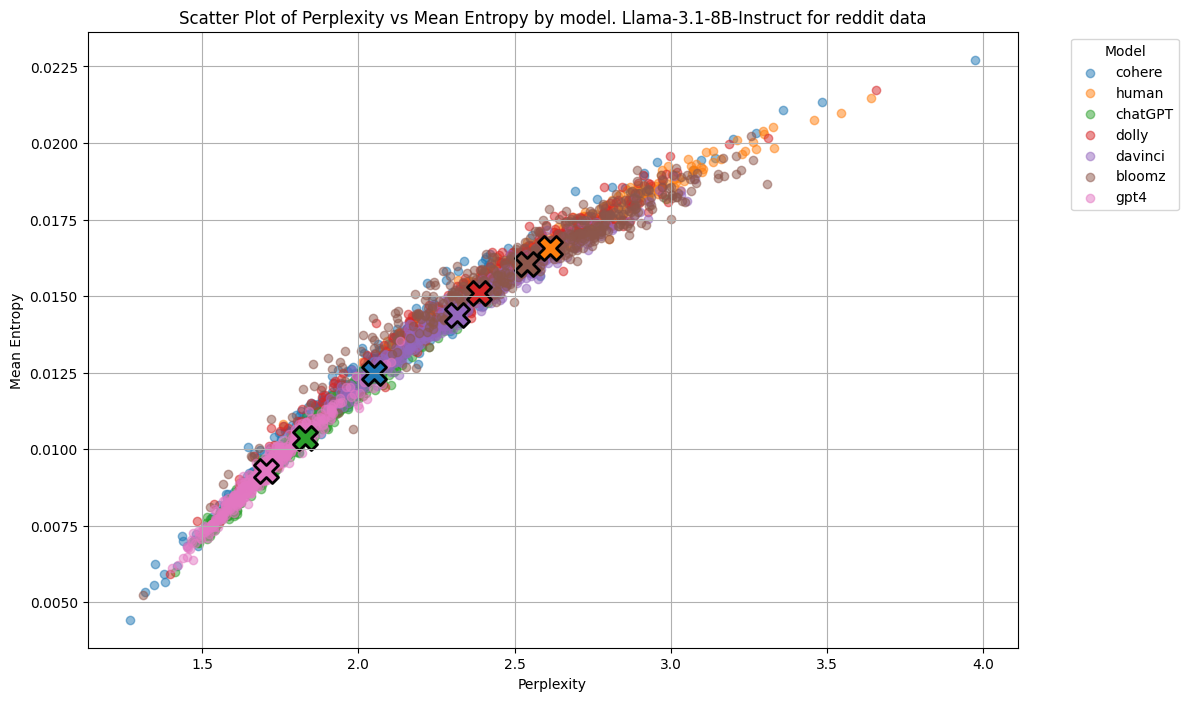
\includegraphics[width=1\textwidth]{reddit.png}   

Texts for different models are clustered by perplexity, and many of the models have significant differences from human texts. 
\end{frame}
\begin{frame}{Distribution for arxiv data}
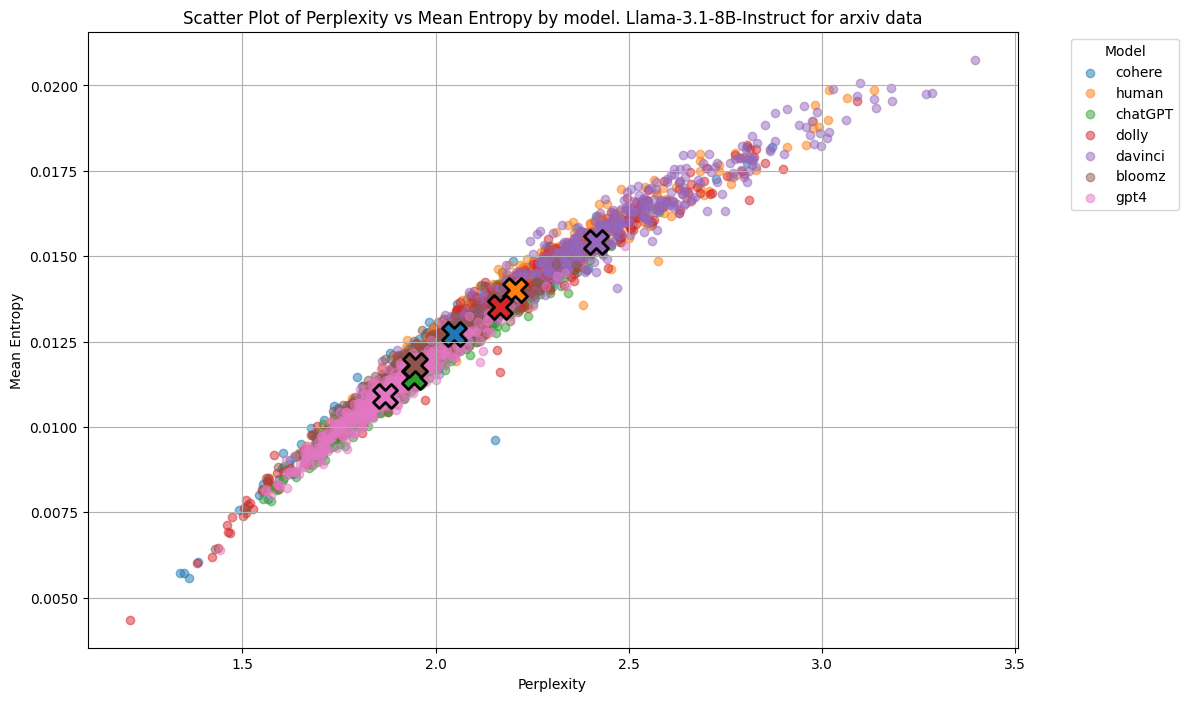
\includegraphics[width=1\textwidth]{arxiv.png}   
\end{frame}
\end{document}
